\section{Terms of SCALE-GM}
%-------------------------------------------------------------------------------

 \begin{itemize}
   \item g-level (grid level): number of subdivision times of the grid from the original icosahedron.
         the number starts from 1, we recommend to use the number larger than 4.
   \item r-level (region level): number of subdivision times of the region(tile)
         from the original icosahedron. When r-level = 0, we have ten regions(tiles).
         At that time, the number of available maximum MPI processes is ten.
 \end{itemize}


%\begin{figure}[H]
%\centering
%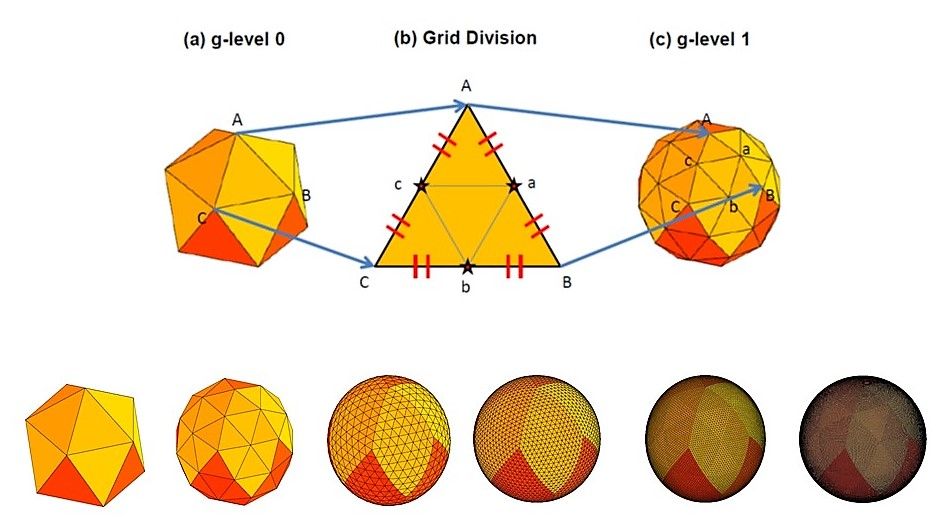
\includegraphics[width=15cm]{g-level_concept.jpg}
%\caption{g-levelの概念図}
%\centering
%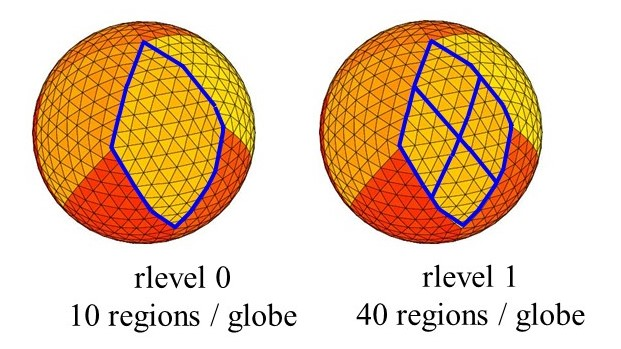
\includegraphics[width=10cm]{r-level_concept.jpg}
%\caption{r-levelの概念図}
%\end{figure}

\textcolor{red}{[要検討: ここに、g-levelとr-levelを説明するための適切な図を追
    加する必要がある:とりあず佐藤さんの発表資料より拝借!さらにHALOを説明する図
    もある方が良い]}

